\begin{figure}[h]
\centering
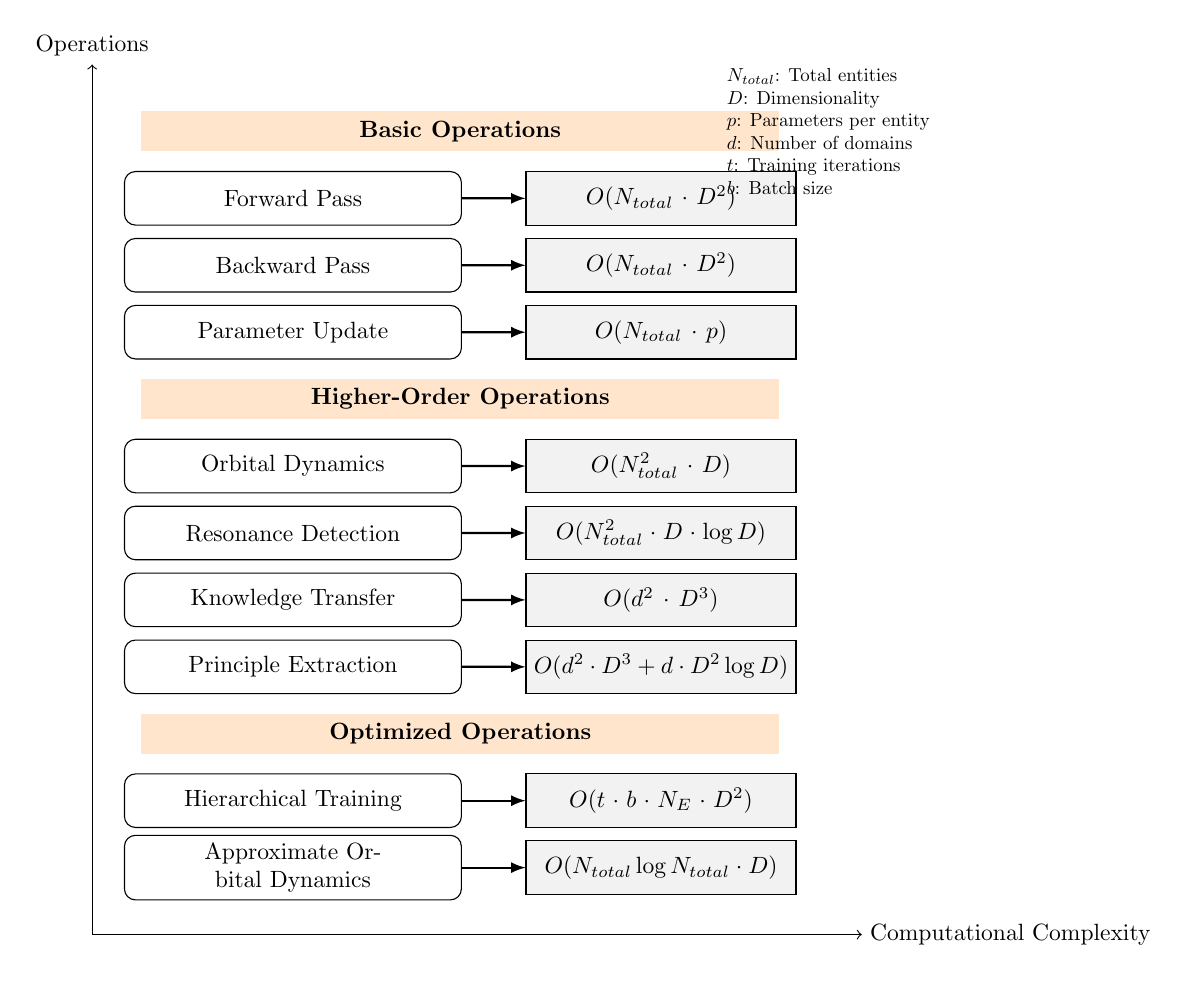
\begin{tikzpicture}[scale=0.85, transform shape]
    % Define styles
    \tikzset{
        operation/.style={draw, rounded corners, minimum width=5cm, minimum height=0.8cm, text width=4.8cm, align=center},
        complexity/.style={draw, fill=gray!10, minimum width=4cm, minimum height=0.8cm, text width=3.8cm, align=center},
        thickarrow/.style={->, >=latex, thick},
        category/.style={draw=none, fill=orange!20, minimum width=9.5cm, minimum height=0.6cm, text width=9.3cm, align=center, font=\bfseries}
    }
    
    % Y-axis (operations)
    \draw[->] (-0.5,0) -- (-0.5,13) node[above] {Operations};
    
    % X-axis (complexity)
    \draw[->] (-0.5,0) -- (11,0) node[right] {Computational Complexity};
    
    % Category 1: Basic Operations
    \node[category] at (5,12) {Basic Operations};
    
    % Operation nodes
    \node[operation] (fwd) at (2.5,11) {Forward Pass};
    \node[operation] (bwd) at (2.5,10) {Backward Pass};
    \node[operation] (upd) at (2.5,9) {Parameter Update};
    
    % Complexity nodes
    \node[complexity] (fwdc) at (8,11) {$O(N_{total} \cdot D^2)$};
    \node[complexity] (bwdc) at (8,10) {$O(N_{total} \cdot D^2)$};
    \node[complexity] (updc) at (8,9) {$O(N_{total} \cdot p)$};
    
    % Arrows
    \draw[thickarrow] (fwd) -- (fwdc);
    \draw[thickarrow] (bwd) -- (bwdc);
    \draw[thickarrow] (upd) -- (updc);
    
    % Category 2: Higher-Order Operations
    \node[category] at (5,8) {Higher-Order Operations};
    
    % Operation nodes
    \node[operation] (orb) at (2.5,7) {Orbital Dynamics};
    \node[operation] (res) at (2.5,6) {Resonance Detection};
    \node[operation] (kt) at (2.5,5) {Knowledge Transfer};
    \node[operation] (pe) at (2.5,4) {Principle Extraction};
    
    % Complexity nodes
    \node[complexity] (orbc) at (8,7) {$O(N_{total}^2 \cdot D)$};
    \node[complexity] (resc) at (8,6) {$O(N_{total}^2 \cdot D \cdot \log D)$};
    \node[complexity] (ktc) at (8,5) {$O(d^2 \cdot D^3)$};
    \node[complexity] (pec) at (8,4) {$O(d^2 \cdot D^3 + d \cdot D^2 \log D)$};
    
    % Arrows
    \draw[thickarrow] (orb) -- (orbc);
    \draw[thickarrow] (res) -- (resc);
    \draw[thickarrow] (kt) -- (ktc);
    \draw[thickarrow] (pe) -- (pec);
    
    % Category 3: Optimized Operations
    \node[category] at (5,3) {Optimized Operations};
    
    % Operation nodes
    \node[operation] (htrain) at (2.5,2) {Hierarchical Training};
    \node[operation] (oapprox) at (2.5,1) {Approximate Orbital Dynamics};
    
    % Complexity nodes
    \node[complexity] (htrainc) at (8,2) {$O(t \cdot b \cdot N_E \cdot D^2)$};
    \node[complexity] (oapproxc) at (8,1) {$O(N_{total} \log N_{total} \cdot D)$};
    
    % Arrows
    \draw[thickarrow] (htrain) -- (htrainc);
    \draw[thickarrow] (oapprox) -- (oapproxc);
    
    % Legend
    \node[align=left, scale=0.8] at (10.5,12) {
        $N_{total}$: Total entities\\
        $D$: Dimensionality\\
        $p$: Parameters per entity\\
        $d$: Number of domains\\
        $t$: Training iterations\\
        $b$: Batch size
    };
    
\end{tikzpicture}
\caption{Computational complexity comparison of key operations in the Elder Heliosystem. The chart shows asymptotic time complexity for basic operations, higher-order operations, and operations with optimized implementations. The complexity is expressed in terms of key system parameters including the total number of entities ($N_{total}$), dimensionality ($D$), number of parameters ($p$), number of domains ($d$), training iterations ($t$), and batch size ($b$).}
\label{fig:complexity_comparison}
\end{figure}